\newpage
\section{Metodologia Experimental}

\subsection{Materiais}

Para a realização do experimento foi utilizado o software Simulink do pacote 
Matlab.

\subsection{Métodos}
O experimento foi realizado em duas simulações. De início, foi estudado o 
comportamento do sistema OFDM com modulação 16-QAM. Em seguida, foi analisada a modulação 4-QAM, de modo a avaliar qual o melhor esquema de modulação, de acordo com o critério da taxa de erro de bit.

As seções seguintes dão mais detalhes sobre o procedimento.

\subsubsection{Simulação com 16-QAM}
Na primeira atividade, foi montado o circuito da figura \ref{fig:16sch}. Os parâmetros de cada bloco são apresentados na figura \ref{fig:dados}.

\begin{figure}[H]
  \centering
  \caption{Diagrama do sistema OFDM com modulação 16-QAM.}
  \includegraphics[scale=1]{16/sch}
  \label{fig:16sch}
    
  \small Fonte: Jacob, J. L., Universidade Estadual de Londrina (2015).
\end{figure}

\begin{figure}[H]
  \centering
  \caption{Parâmetros do sistema 16-QAM.}
  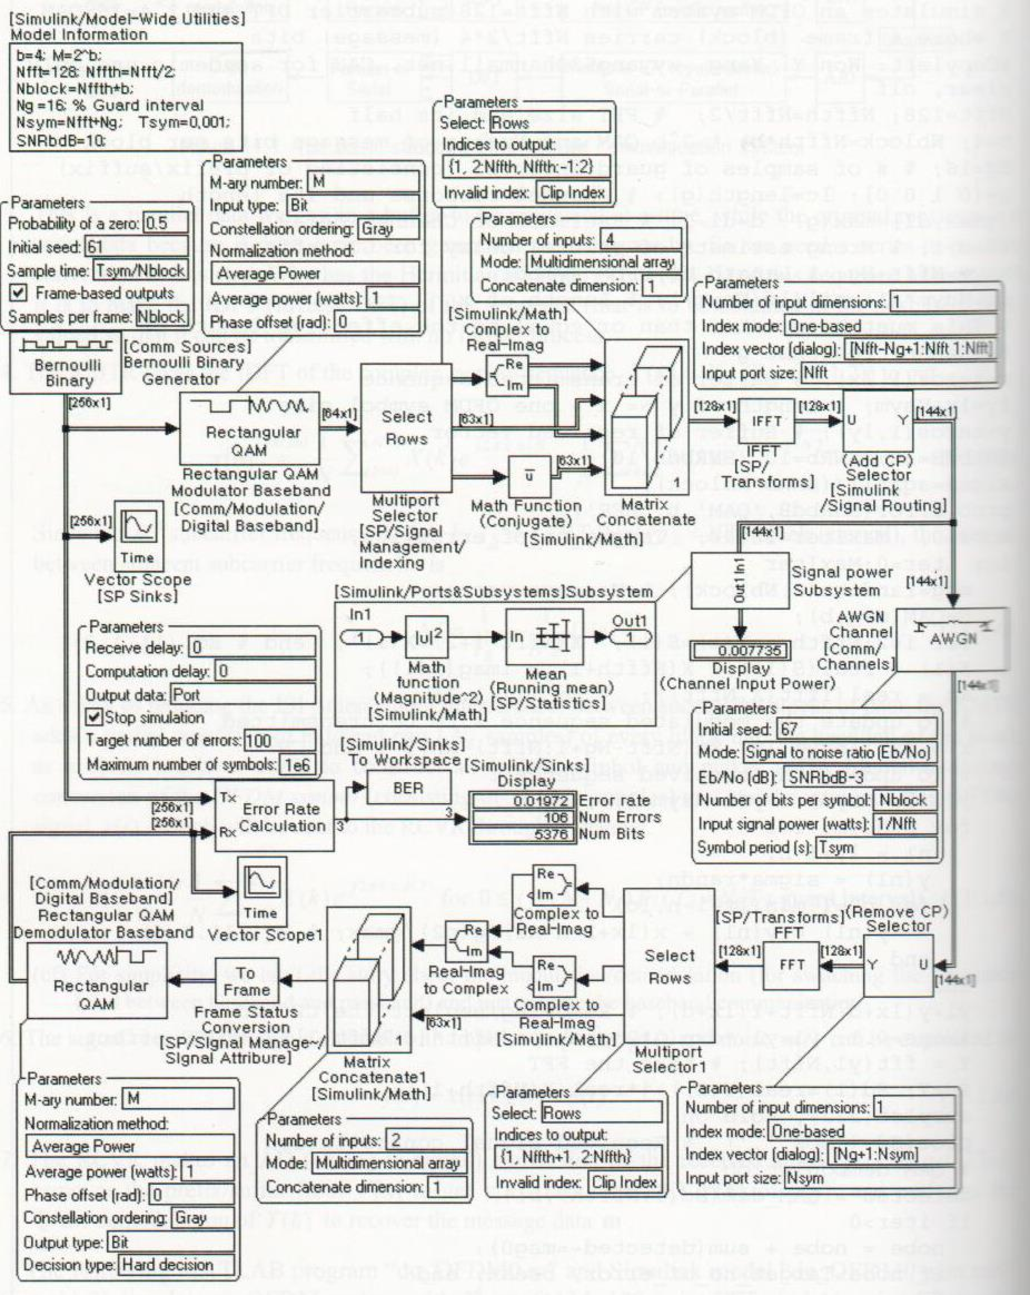
\includegraphics[scale=1]{dados}
  \label{fig:dados}
  
  \small Fonte: Jacob, J. L., Universidade Estadual de Londrina (2015).
\end{figure}

Foram obtidos:

\begin{enumerate}
  \item os espectros de 1, 2 e 3 e a constelação 1. Também a constelação 2, para $\frac{E_b}{N_0} = 20 dB$ e $\frac{E_b}{N_0} = 0 dB$;
  
  \item gráficos nos osciloscópios Scope e Scope 1, para $\frac{E_b}{N_0} = 12 dB$;
  
  \item o gráfico da BERxEb/No, após do preenchimento da tabela \ref{tab:ber16}.
\end{enumerate}

\begin{table}[H]
  \begin{center}
    \caption{Tabela BER x Eb/No para 16-QAM.}
    \begin{tabular}{ccc}
      \toprule
      $\frac{E_b}{N_0}$ (dB) & BER \\
      \midrule
      10 & 3.39e-3 \\
      8 &  \\
      6 & \\
      4 & \\
      2 & \\
      0 & \\
      -2 & \\
      \bottomrule
    \end{tabular}
    \label{tab:ber16}
  \end{center}
\end{table}

\subsubsection{Simulação com 4-QAM}

Na segunda atividade, foi montado o circuito da figura \ref{fig:4sch}. Os parâmetros de cada bloco são os mesmos, porém, com b =2.

\begin{figure}[H]
  \centering
  \caption{Diagrama do sistema OFDM com modulação 4-QAM.}
  \includegraphics[scale=0.8]{4/sch}
  \label{fig:4sch}
  
  \small Fonte: Jacob, J. L., Universidade Estadual de Londrina (2015).
\end{figure}

Foram obtidos:

\begin{enumerate}
  \item a constelação 1. Também a constelação 2, para $\frac{E_b}{N_0} = 20 dB$ e $\frac{E_b}{N_0} = 0 dB$;
  
  \item gráficos nos osciloscópios Scope e Scope 1, para $\frac{E_b}{N_0} = 12 dB$;
  
  \item o gráfico da BERxEb/No, após do preenchimento da tabela \ref{tab:ber4}.
\end{enumerate}

\begin{table}[H]
  \begin{center}
    \caption{Tabela BER x Eb/No para 4-QAM.}
    \begin{tabular}{ccc}
      \toprule
      $\frac{E_b}{N_0}$ (dB) & BER \\
      \midrule
      8 & 6.23e-4 \\
      6 & \\
      4 & \\
      2 & \\
      0 & \\
      -2 & \\
      \bottomrule
    \end{tabular}
    \label{tab:ber4}
  \end{center}
\end{table}

\subsection{Comparação entre 16-QAM e 4-QAM}
Foi realizada uma comparação entre os resultados obtidos para modulação 16-QAM e 4-QAM através do gráfico da BERxEb/No para os dois sistemas.

